\documentclass{standalone}
\usepackage{tikz}

\usetikzlibrary{shapes, arrows, babel}
\tikzstyle{bloque}=[draw, rectangle, 
minimum height=3em, minimum width=6em]
\tikzstyle{suma}=[draw, circle, node distance=1cm]
\tikzstyle{entrada}=[coordinate]
\tikzstyle{salida}=[coordinate]
\tikzstyle{pinstyle}=[pin edge={to-, thin, black}]

\begin{document}
	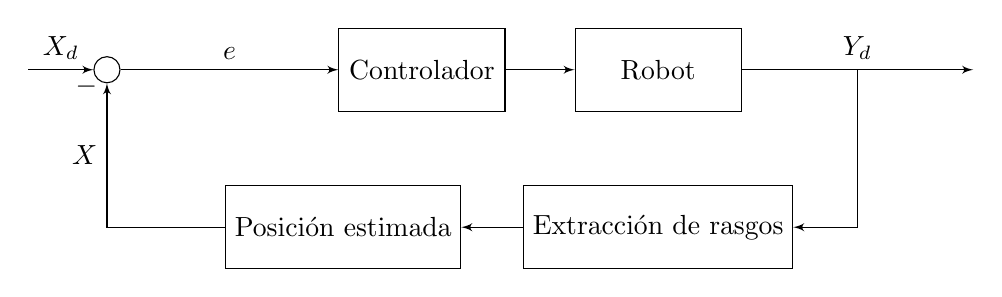
\begin{tikzpicture}[auto, node distance=4cm, >=latex']
		\node[entrada, name=entrada]{};
		\node[suma, right of=entrada](suma){};
		\node[bloque, right of=suma](control){Controlador};
		\node [bloque, right of=control, node distance=3cm](sistema){Robot}; 
		\draw[->] (control) -- node[name=u] {} (sistema);
		\node[salida, right of=sistema](salida){};
		\node[bloque, below of=sistema, node distance=2cm](sensor){Extracci\'on de rasgos}; 
		\node[bloque, left of=sensor](posi){Posici\'on estimada};
		\draw [draw,->] (entrada) -- node {$X_{d}$} (suma);
		\draw [->] (suma) -- node {$e$} (control);
		\draw [->] (sistema) -- node [name=y] {$Y_{d}$}(salida);
		\draw [->] (y) |- (sensor);
		\draw[->] (sensor) -- node{} (posi);
		\draw [->] (posi) -| node[pos=0.99] {$-$} 
		node [near end] {$X$} (suma);
	\end{tikzpicture}
\end{document}